\documentclass[shortlabels]{article}
\usepackage{import}
\subimport*{./}{macro}

\usepackage[ruled]{algorithm2e}

\setlength\parindent{0px}

\begin{document}
\setcounter{aprob}{0}
\setcounter{bprob}{0}
\title{Homework \#2}
\author{
    \normalsize{CSE 446/546: Machine Learning}\\
    \normalsize{Profs. Jamie Morgenstern and Simon Du}\\
    \normalsize{Due: \textbf{Wednesday} November 3, 2021 11:59pm}\\
    \normalsize{\textbf{A:} 96 points, \textbf{B:} 29 points} \\
    \normalsize{Sami Turbeville, \textbf{Collab:} Shabab Ahmed}
    }
\date{{}}
\maketitle

\section*{Short Answer and ``True or False'' Conceptual questions}

\begin{aprob}
    The answers to these questions should be answerable without referring to external materials.  Briefly justify your answers with a few words.
    \begin{enumerate}
      \item \points{2} Suppose that your estimated model for predicting house prices has a large positive weight on the feature \texttt{number of bathrooms}. If we remove this feature and refit the model, will the new model have a strictly higher error than before? Why?

      \textbf{Solution:} No,  the error won't necessarily increase if there is a correlated parameter such as \texttt{number of showers}, then the weight increases for the \texttt{number of showers}. But if they are are not perfectly correlated then the error will increase.
      \newpage
      \item \points{2} Compared to L2 norm penalty, explain why a L1 norm penalty is more likely to result in sparsity (a larger number of 0s) in the weight vector.

      \textbf{Solution:} L1 has the objective $$ \text{min}_w \text{RSS} + \lambda \| w \|_1$$ whereas the L2 objective is $$ \text{min}_w \text{RSS} + \lambda \| w \|_2^2 $$ Graphically denoted in Figure 13.3 in the textbook. As you can see graphically, as the L1 and L2 balls grow then they are likely to intersect with the constraint in different spots - L1 is preferred to intersect at the spike or corner at 0 causing the matrix to be sparce but the L2 ball is not going to intersect the constraint at 0 since it is a circle there is no preferred sparce intersection. 
      \newpage
      \item \points{2} In at most one sentence each, state one possible upside and one possible downside of using the following regularizer: $\left(\sum_{i}\left|w_{i}\right|^{0.5}\right)$.

      \textbf{Solution:} Pro: It is more sparse. Con: It is not convex.
      \newpage
      \item \points{1} True or False: If the step-size for gradient descent is too large, it may not converge.

      \textbf{Solution:} True, if the step size is too large then it may miss the minimum point.
      \newpage
      \item \points{2} In your own words, describe why stochastic gradient descent (SGD) works, even though only a small portion of the data is considered at each update.

      \textbf{Solution:} It works because it finds the minimum using a random point, then based on the slope of the function for each dimension/feature it finds a new point to test to see if the gradient is zero. Using a reasonably small step size, we can confidently narrow down our gradient or slope until it is near zero. This is much more efficient and less work than finding the derivative at each point then the gradient descent method.
      \newpage
      \item \points{2} In at most one sentence each, state one possible advantage of SGD over GD (gradient descent), and one possible disadvantage of SGD relative to GD.

        \textbf{Solution:} One advantage to SGD is the computational efficiency - it needs to do much less computations for each step in the SGD compared to GD. One disadvantage is that it might be noisier and not exactly at the minimum point in the function.
    \end{enumerate}

\end{aprob}

\newpage

\section*{Convexity and Norms }

\begin{aprob}
    A \emph{norm} $\|\cdot\|$ over $\R^n$ is defined by the properties:
    (\textit{i}) non-negativity: $\|x\|\geq 0$ for all $x \in \R^n$ with equality if and only if $x=0$,
    (\textit{ii}) absolute scalability: $\|a \, x\| = |a| \, \|x\|$ for all $a \in \R$ and $x \in \R^n$,
    (\textit{iii}) triangle inequality: $\|x+y\| \leq \|x\| + \|y\|$ for all $x,y \in \R^n$.
    \begin{enumerate}
      \item \points{3} Show that $f(x) = \left( \sum_{i=1}^n |x_i| \right)$ is a norm. (Hint: for (\textit{iii}), begin by showing that $|a+b|\leq |a| + |b|$ for all $a,b \in \R$.)
      \item \points{2} Show that $g(x) = \left(\sum_{i=1}^n |x_i|^{1/2}\right)^2$ is not a norm. (Hint: it suffices to find two points in $n=2$ dimensions such that the triangle inequality does not hold.)
    \end{enumerate}
    Context: norms are often used in regularization to encourage specific behaviors of solutions. If we define  $\| x \|_p := \left( \sum_{i=1}^n |x_i|^{p} \right)^{1/p}$ then one can show that $\| x \|_p$ is a norm for all $p \geq 1$. The important cases of $p=2$ and $p=1$ correspond to the penalty for ridge regression and the lasso, respectively. \\

    \subsection*{Solutions:}
    \begin{enumerate}
        \item
        \begin{proof}
            We will show that $f(x) = \left( \sum_{i=1}^n |x_i| \right)$ is a norm. We will show all three properties of norms listed above hold.

            (i) For all $x \in \R^n$, the absolute value of $x_i$ is non-negative. It follows that the sum of a non-negative number is non-negative. So $f(x) = \left( \sum_{i=1}^n |x_i| \right) \geq 0$ with equality when $\vec{x} = \vec{0}$ since $f$ is the sum of absolute values of each element of $\vec{x}$ and no element is negative so it can only be that we have equality when $\vec{x} = \vec{0}$.

            (ii) We will show scalability ($f(ax) = a \cdot f(x)$) for all $a \in \R$ and $x \in \R^n$.
            \[ f(ax) = \left( \sum_{i=1}^n |a x_i| \right) \] 
            By linearity of the summation,
            \[ =  \left( |a| \sum_{i=1}^n |x_i| \right) = a \cdot f(x) \]

            (iii)
            For all $x,y \in \R^n$, we will show that $ f(x + y)  \leq  f(x)  + f(y) $.
            \[  f(x)  +  f(y)  =  \sum_{i=1}^n |x_i|  +  \sum_{i=1}^n |y_i|  \]
            By linearity and because the norm is the absolute value for $x_i \in \R$, 
            \[  = \sum^n_{i=1} \left( |x_i| + |y_i| \right) \] 
            where for each $i$, the triangle inequality holds for $x_i, y_i \in \R$.
            \[ |x_i| + |y_i| \geq | x_i + y_i | \]
            Then,
            $$ \sum^n_{i=1} \left( |x_i| + |y_i| \right) \geq  \sum^n_{i=1} \left( |x_i + y_i | \right) $$
            where 
            $$ \sum^n_{i=1} \left( |x_i + y_i | \right) =  f(x  +  y) $$
            Thus, $  f(x+y) \leq f(x) + f(y) $,  the triangle inequality holds for $f(x)$ as shown.
        \end{proof}
        \newpage
        \item \begin{proof}
            We will prove by counter example in dimension of 2. For $x,y \in \R^2$, $g$ is not a norm because the triangle inequilty does not hold. 
            For example, when $x = [ 0.2, 0.1 ]$ and $y = [ 4,8]$ then $$g(x+y) = 23.97 \nleq g(x) + g(y) = 23.89$$.
        \end{proof}
    \end{enumerate}
\end{aprob}

\newpage


\begin{bprob}
    A set $A \subseteq \R^n$ is \emph{convex} if $\lambda x + (1-\lambda) y \in A$ for all $x,y\in A$ and $\lambda \in [0,1]$. Let $\| \cdot \|$ be a norm.
    \begin{enumerate}
        \item \points{3} Show that $f(x) = \| x \|$ is a convex function.
        
        \begin{proof}
            We will show that the norm $f(x) = \| x \|$ is a convex function. Let $x,y  \in A$ then we will show that $f(\lambda x + (1-\lambda) y )\leq \lambda f(x) + (1-\lambda) f(y)$ where $\lambda \in [0,1]$.
            \begin{align*}
                f(\lambda x + (1-\lambda) y ) &= \| \lambda x + (1-\lambda) y \| \\
                &\leq \| \lambda x \| + \| (1-\lambda) y \| \ \ \text{by triangle inequality}\\
                &= |\lambda| \|x\| + | 1 - \lambda | \| y \|  \\
                &= \lambda \|x\| + (1 - \lambda) \| y \| \ \ \text{since }\lambda \in [0,1]\\ 
                &= \lambda f(x) + (1-\lambda) f(y)
            \end{align*}
        Therefore, $f(x) = \| x \|$ is convex.
        \end{proof}
        \newpage

        \item \points{3} Show that $\{ x \in \R^n : \|x\| \leq 1\}$ is a convex set.

        \begin{proof}
            Similar to previous problem, we will show that $\{ x \in \R^n : \|x\| \leq 1\}$ is a convex set. Let $a,b \in \R$ where $\|a\| \leq 1$ and $\|b\| \leq 1$.
            \begin{align*}
                \| \lambda a + (1-\lambda) b \| 
                 &\leq \| \lambda a \| + \| (1-\lambda) b \| \ \ \text{by triangle inequality}\\
                \implies &= |\lambda| \|x\| + | 1 - \lambda | \| y \|  \\
                \implies &= \lambda \|a\| + (1 - \lambda) \| b \| \ \ \text{since }\lambda \in [0,1]\\
                \implies &\leq \lambda  + (1-\lambda)  \ \ \text{ using largest possible value for a and b = 1} \\
                \implies &= 1 \\
            \end{align*}
            Thus, $\| \lambda a + (1-\lambda) b \| \leq 1$. So the set is convex.
            \end{proof}
        
        \newpage

        \item \points{2} Draw a picture of the set $\{ (x_1,x_2) ~: ~ g(x_1,x_2) \le 4 \}$
        where $g(x_1, x_2)  = \left( |x_1|^{1/2} + |x_2|^{1/2}\right)^2$. (This is the function considered in 1b above specialized to $n=2$.) We know $g$ is not a norm. Is the defined set convex? Why not?
    
        Let us draw the set (used wolfram alpha):

        % \begin{figure}[h]
            \centering
            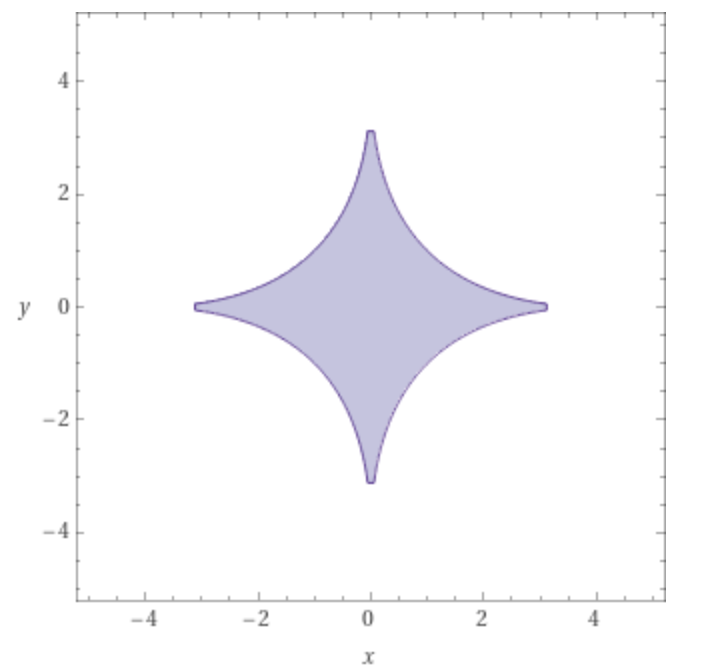
\includegraphics[width=0.3\textwidth]{../hw2-code/convex_sets_B1.png}
            % \caption{blah}
            % \label{fig:concave_set}
        % \end{figure}


        Visually, you can see this set is not concave. We prove that here: 
        \begin{proof}
        Let
        $x_1 = [0,4]$ and $x_2 = [4,0]$ which are in the set. If the set were convex, 
        then $\lambda x_1 + (1-\lambda) x_2 $ would also be in the set ($\leq 4$) for all $\lambda \in [0,1]$.
        Let $\lambda = 0.5$ then,
        $$ \lambda x_1 + (1-\lambda) x_2 = 0.5 \cdot [0,1] + (0.5) [1,0] = [2, 2] $$
        $$ g(2,2) = (\sqrt(2)+\sqrt(2))^2 = 8 \nleq 4 $$
        So $g$ is not a convex set.
        \end{proof}

    \end{enumerate}
    Context: It is a fact that a function $f$ defined over a set $A \subseteq \R^n$ is convex if and only if the set $\{ (x, z) \in \R^{n+1} : z \geq f(x), x \in A \}$ is convex. Draw a picture of this for yourself to be sure you understand it.

\end{bprob}
\newpage
\begin{bprob}
    For $i=1,\dots,n$ let $\ell_i(w)$ be convex functions over $w \in \R^d$ (e.g., $\ell_i(w) = (y_i - w^\top x_i)^2$), $\| \cdot \|$ is any norm, and $\lambda >0$. 
    \begin{enumerate}
        \item \points{3} Show that 
        \begin{align*}
            \sum_{i=1}^n \ell_i(w) + \lambda \| w \|
        \end{align*}
        is convex over $w\in \R^d$ (Hint: Show that if $f,g$ are convex functions, then $f(x) + g(x)$ is also convex.) 
        
        \begin{proof}
            We will first show by induction that $\sum_{i=1}^n \ell_i(w)$ is convex. Then we will show that $\sum_{i=1}^n \ell_i(w) + \lambda \| w \| $ is convex.

            \textbf{Base Case:}$(k=2)$ Show that $\ell_1 + \ell_2$ is convex. 
            We will show that $(\ell_1 + \ell_2)(w) = \ell_1(w) + \ell_2(w)$ for some $w \in \R^d$. Let $\lambda >0$ then,
            \begin{align*}
                (\ell_1 + \ell_2)(\lambda x + (1-\lambda)y) &= \ell_1(\lambda x + (1-\lambda)y) + \ell_2(\lambda x + (1-\lambda)y) \\
                &\leq \ell_1(\lambda x) + \ell_1((1-\lambda)y) + \ell_2(\lambda x) + \ell_2((1-\lambda)y) \\
                \implies &= \lambda \ell_1( x) + (1-\lambda) \ell_1(y) + \lambda  \ell_2(x) + (1-\lambda) \ell_2(y) \\
                \implies &=  \lambda (\ell_1 + \ell_2) (x) + (1-\lambda) (\ell_1 + \ell_2) (y) \\
            \end{align*}
            Thus, $\ell_1 + \ell_2$ is convex.

            Suppose this base case holds true up to $k$. We will show it also holds for $k+1$.
            Then $\sum_{i=1}^k (l_i(w))$ is convex, we will show $\sum_{i=1}^{k+1} (l_i(w))$ is also convex.
            Let's break this down:
            $$ \sum_{i=1}^{k+1} (l_i(w)) = \sum_{i=1}^k (l_i(w)) + l_{k+1}(w)$$
            By the base case, the sum of two convex sets is convex so $\sum_{i=1}^{k+1} (l_i(w))$ by induction.
        \end{proof}

        \newpage

        \item \points{1} Explain in one sentence why we prefer to use loss functions and regularized loss functions that are convex.
    
        \textbf{Solution:} Convex sets are usually easier to work with due to their properties and that the minima of a convex function is the global minima so our gradient descent algorithms will always find the global minima. 
    \end{enumerate}

\end{bprob}

\newpage

\section*{Lasso on a Real Dataset}

\subsection*{A Lasso Algorithm}
Given $\lambda >0$ and data $\Big (x_i,y_i \Big)_{i=1}^n$, the Lasso is the problem of solving
\begin{equation*}\label{eq:lasso}
  \arg\min_{{w}\in \R^d, b \in \R} \sum_{i=1}^n { (x_i^T {w} + b - {y}_i)^2 }
    + \lambda \sum_{j=1}^d |{w}_j|
\end{equation*}
where $\lambda$ is a regularization parameter.
For the programming part of this homework, we have implemented the coordinate descent method shown in Algorithm~\ref{alg:cd} to solve the Lasso problem for you.

\begin{algorithm}[h]
    \caption{Coordinate Descent Algorithm for Lasso}\label{alg:cd}
    \While{not converged}{
      $b \leftarrow \frac{1}{n}\sum_{i=1}^n \left({y}_i - \sum_{j=1}^d {w}_j {x}_{i,j}\right)$\\ 
      \For{$k \in \{1,2,\cdots d\}$} {
        $a_k\leftarrow 2 \sum_{i=1}^n {x}_{i,k}^2$ \\   
        $c_k\leftarrow 2 \sum_{i=1}^n {x}_{i,k} \left({y}_i -(b + \sum_{j\neq k} {w}_j {x}_{i,j} )\right)$ \\
        ${w}_k \leftarrow
        \left\{
        \begin{array}{ll}
          (c_k+\lambda) / a_k & c_k < -\lambda\\
          0 & c_k\in [-\lambda, \lambda]\\
          (c_k-\lambda) / a_k & c_k > \lambda\\
        \end{array}
        \right.
        $
      }
    }
\end{algorithm}

    You will often apply Lasso on the same dataset for many values of $\lambda$.  This
    is called a regularization path.  One way to do this efficiently is to start at a large $\lambda$, and then for each consecutive solution, initialize the algorithm with the previous solution, decreasing $\lambda$ by a constant ratio (e.g., by a factor of $2$).

  The smallest value of $\lambda$ for which the solution $\widehat{w}$ is entirely zero is given by
       \begin{align}
           \lambda_{max} = \max_{k=1,\dots,d} 2 \left|\sum_{i=1}^n {x}_{i,k} \left({y}_i - \left(\frac{1}{n} \sum_{j=1}^n y_j \right)\right)\right|\label{eqn:lasso-lambdamax}
       \end{align}
      This is helpful for choosing the first $\lambda$ in a regularization path. 

    A benefit of the Lasso is that if we believe many features are irrelevant for predicting ${y}$, the Lasso can be used to enforce a sparse solution, effectively differentiating between the relevant and irrelevant features.

    \newpage

    \subsection*{Dataset}

    Download the training data set ``crime-train.txt'' and the test data set ``crime-test.txt'' from the course website. Store your data in your working directory, ensure you have \texttt{pandas} installed, and read in the files with the following Python code:

    \begin{verbatim}
        import pandas as pd
        df_train = pd.read_table("crime-train.txt")
        df_test = pd.read_table("crime-test.txt")
    \end{verbatim}

    This stores the data as Pandas \texttt{DataFrame} objects. \texttt{DataFrame}s are similar to Numpy \texttt{array}s but more flexible; unlike \texttt{array}s, \texttt{DataFrame}s store row and column indices along with the values of the data. Each column of a \texttt{DataFrame} can also store data of a different type (here, all data are floats). 

    Here are a few commands that will get you working with Pandas for this assignment:

    \begin{verbatim}
        df.head()                   # Print the first few lines of DataFrame df.
        df.index                    # Get the row indices for df.
        df.columns                  # Get the column indices.
        df[``foo'']                # Return the column named ``foo''.
        df.drop(``foo'', axis = 1)  # Return all columns except ``foo''.
        df.values                   # Return the values as a Numpy array.
        df[``foo''].values         # Grab column foo and convert to Numpy array.
        df.iloc[:3,:3]              # Use numerical indices (like Numpy) to get 3 rows and cols.
    \end{verbatim}

    The data consist of local crime statistics for 1,994 US communities. The response $y$ is the rate of violent crimes reported per capita in a community. The name of the response variable is \texttt{ViolentCrimesPerPop}, and it is held in the first column of \texttt{df\_train} and \texttt{df\_test}. There are 95 features. These
    features include many variables.

    Some features are the consequence of complex political processes, such as the size of the police force and other systemic and historical factors. Others are demographic
    characteristics of the community, including self-reported statistics about race, age, education, and employment drawn from Census reports.\\

    The dataset is split into a training and test set with 1,595 and 399 entries, respectively. The features have been standardized to have mean 0 and variance 1. 
    We will use this training set to fit a model to predict the crime rate in new communities and evaluate model performance on the test set.  As there are a considerable number of input variables and fairly few training observations, overfitting is a serious issue, and the coordinate descent Lasso algorithm may mitigate this problem during training. \\

    The goals of this problem are threefold: ($i$) to encourage you to think about how data collection processes affect the resulting model trained from that data; ($ii$) to encourage you to think deeply about models you might train and how they might be misused; and ($iii$) to see how Lasso encourages sparsity of linear models in settings where $d$ is large relative to $n$. \textbf{We emphasize that training a model on this dataset can suggest a degree of correlation between a community's demographics and the rate at which a community experiences and reports violent crime. We strongly encourage students to consider why these correlations may or may not hold more generally, whether correlations might result from a common cause, and what issues can result in misinterpreting what a model can explain.}\\

\newpage
\subsection*{Applying Lasso}


\begin{aprob}

    \begin{enumerate}
        \item \points{4} Read the documentation for the original version of this dataset: \url{http://archive.ics.uci.edu/ml/datasets/communities+and+crime}. Report 3 features included in this dataset for which historical \emph{policy} choices in the US would lead to variability in these features. As an example, the \emph{number of police} in a community is often the consequence of decisions made by governing bodies, elections, and amount of tax revenue available to decision makers.
        
        \textbf{Solution:}
        There are several variables that would be different if other policy choices were made in the US and specifically in those communities. For example, median income varies based on policy choices like which communities to include low-income housing or waterfront communities with mansions. 
        Another statistic that might changed based on policy decisions is the number of people in homeless shelters or on the street because this number depends on the capacity of the shelters and the policies which determine aid available to homeless individuals to help them get off the street. 
        Population is another metric that can vary based on policy because of the zoning codes for apartment buildings which allow for higher density of people in a community compared to more rural or farm lands that have little commercial and apartment style housing and even redlining.

        \newpage
        \item \points{4} Before you train a model, describe 3 features in the dataset which might, if found to have nonzero weight in model, be interpreted as \emph{reasons} for higher levels of violent crime, but which might actually be a \emph{result} rather than (or in addition to being) the cause of this violence.
    
        \textbf{Solution:}
        Median income - if there is a lot of violent crime in a community, if they are able (have the financial means) to people will move out of that area so the median income will decrease as a result of increased violent crimes. 
        Similiarly, the number of vacant houses may increase and owner occupied houses may decrease becacuse the neighborhood is less desireable for more wealthy people, leaving the people who are unable to afford a nicer and safer community. 
        Even the percent of black residents may increase in a neighborhood with higher crime rates for the same reason as median income and owner occupied houses decrease. 
    \end{enumerate}

    \newpage

    Now, we will run the Lasso solver. Begin with $\lambda = \lambda_{\max}$ defined in Equation \eqref{eqn:lasso-lambdamax}. Initialize all weights to $0$. Then, reduce $\lambda$ by a factor of 2 and run again, but this time initialize $\hat{{w}}$ from your $\lambda = \lambda_{\max}$ solution as your initial weights, as described above. Continue the process of reducing $\lambda$ by a factor of 2 until $\lambda < 0.01$.
    For all plots use a log-scale for the $\lambda$ dimension (Tip: use
    \verb|plt.xscale('log')|).
    \\


    \begin{enumerate}
        \item[c.] \points{4} Plot the number of nonzero weights of each solution as a function of $\lambda$.
        \begin{figure}[h]
            \centering
            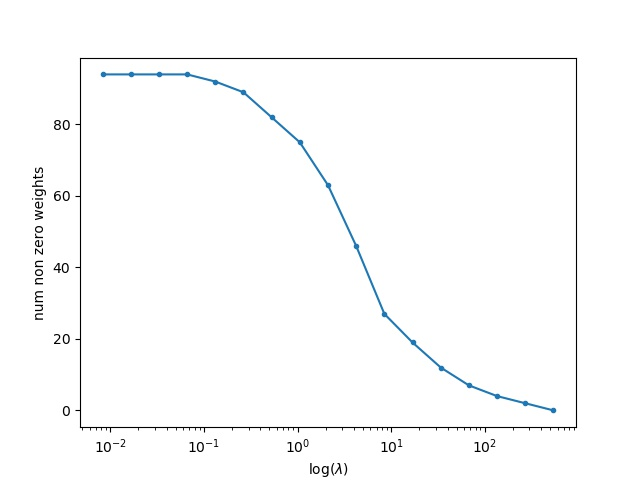
\includegraphics[width=0.5\textwidth]{../hw2-code/lambda_vs_num-nonzero.jpg}
            \caption{Shows number of nonzero weights of each solution as a function of $\lambda$.}
            \label{fig:num_nonzero}
        \end{figure}
        \newpage
        \item[d.] \points{4} Plot the regularization paths (in one plot) for the coefficients for input variables \texttt{agePct12t29}, \texttt{pctWSocSec}, \texttt{pctUrban}, \texttt{agePct65up}, and \texttt{householdsize}.
        \begin{figure}[h]
            \centering
            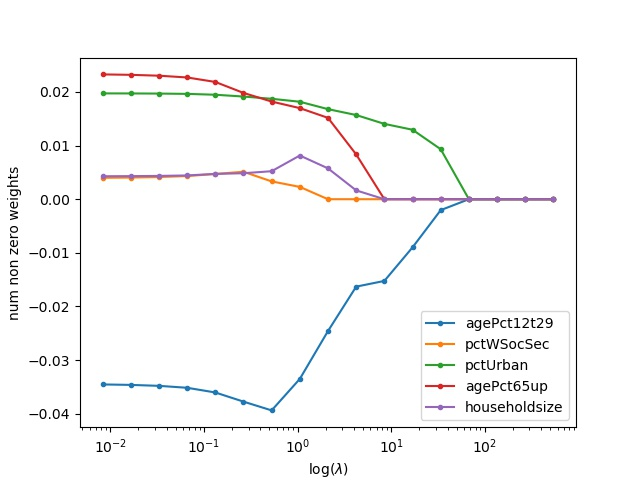
\includegraphics[width=0.5\textwidth]{../hw2-code/lambda_vs_regularizationpaths.jpg}
            \caption{Shows the regularizaiton paths (or weights) for the coeffifients or features labeled 
            \texttt{agePct12t29}, \texttt{pctWSocSec}, \texttt{pctUrban}, \texttt{agePct65up}, and \texttt{householdsize}.}
            \label{fig:regularizationpaths}
        \end{figure}
        \newpage
        \item[e.] \points{4} On one plot, plot the squared error on the training and test data as a function of $\lambda$.
        \begin{figure}[h]
            \centering
            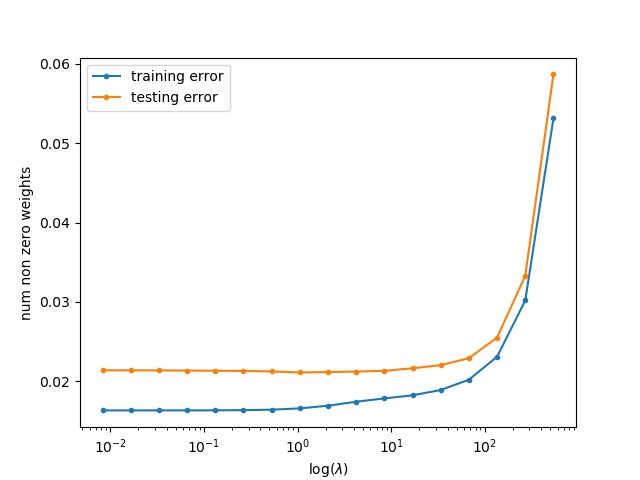
\includegraphics[width=0.5\textwidth]{../hw2-code/lambda_vs_sq-er.jpg}
            \caption{Shows the mean squared error on the training and test data as a function of $\lambda$.}
            \label{fig:squared_error}
        \end{figure}
        \newpage
        \item[f.] \points{4} Sometimes a larger value of $\lambda$ performs nearly as well as a smaller value, but a larger value will select fewer variables and perhaps be more interpretable.  Inspect the weights $\hat{w}$ for $\lambda = 30$.  Which feature had the largest (most positive) Lasso coefficient? What about the most negative? Discuss briefly.
        
        For $\lambda = 30$, there are only 12 nonzero weights: \texttt{agePct12t29, pctUrban, MalePctDivorce, PctKids2Par,
        PctWorkMom, PctIlleg, PctPersDenseHous, HousVacant,
        PctHousOccup, PctVacantBoarded, NumStreet,} and \texttt{LemasPctOfficDrugUn}. The feature with the largest positive weight is \texttt{PctIlleg}.
        The largest negative weight is \texttt{PctKids2Par}. As we discussed in part b, the number of illegal immigrants could be a result of the high violent crime rate rather than causing it. Similarly, if there is a lot of violent crime the amount of children with 2 parents will be lower since dual income parents would likely move out of the commumity to a safer area, reducing the amount of kids with 2 parents, leaving those who cannot afford to move out (single parents).
        
        \newpage
        \item[g.] \points{4} Suppose there was a large negative weight on \texttt{agePct65up} and upon seeing this result, a politician suggests policies that encourage people over the age of 65 to move to high crime areas in an effort to reduce crime. What is the (statistical) flaw in this line of reasoning? (Hint: fire trucks
        are often seen around burning buildings, do fire trucks cause fire?)
    
        If there were a large negative weight on \texttt{agePct65up} does not necessarily cause the high crime rate - it is just highly correlated. Obviously this politician does not know that correlation is not causation. It could be that senior citizens chose not to retire in a neighborhood with high crime rates after having worked their whole lives, they want to retire in peace (aka move to Florida).
    \end{enumerate}
    \newpage
\end{aprob}

\section*{Logistic Regression}
\subsection*{Binary Logistic Regression}
\begin{aprob}
    Here we consider the MNIST dataset, but for binary classification. Specifically, the task is to determine whether a digit is a $2$ or $7$.
    Here, let $Y=1$ for all the ``7'' digits in the dataset, and use $Y=-1$ for ``2''.
    We will use regularized logistic regression. 
    Given a binary classification dataset $\{(x_i,y_i)\}_{i=1}^n$ for $x_i \in \R^d$ and $y_i \in \{-1,1\}$ we showed in class that the regularized negative log likelihood objective function can be written as
    
    \begin{align*}
        J(w,b) = \frac{1}{n} \sum_{i=1}^n \log( 1 + \exp(-y_i (b + x_i^T w))) + \lambda ||w||_2^2
    \end{align*}

    Note that the offset term $b$ is not regularized. 
    For all experiments, use $\lambda = 10^{-1}$. 
    Let $\mu_i(w,b) = \frac{1}{1+ \exp(-y_i (b + x_i^T w))}$. 
    \begin{enumerate}
        \item \points{8} Derive the gradients $\nabla_w J(w,b)$, $\nabla_{b} J(w,b)$ and give your answers in terms of $\mu_i(w,b)$ (your answers should not contain exponentials).
        \subsubsection*{Solution:} 
        \begin{align*}
            \nabla_w J(w,b) = \frac{\diff}{\diff w} \frac{1}{n} \sum_{i=1}^n \log( 1 + \exp(-y_i (b + x_i^T w))) + \lambda ||w||_2^2
        \end{align*}
        Let's ignore the summation for now and focus on the interior:
        \begin{align*}
            \frac{\diff}{\diff w} & \log( 1 + \exp(-y_i (b + x_i^T w))) + \lambda ||w||_2^2 \\
            \frac{\diff}{\diff w} & \log( 1 + \exp(-y_i (b + x_i^T w))) + \frac{\diff}{\diff w} \lambda ||w||_2^2 \\
        \end{align*}
        Let $\mu_i(w,b) = \frac{1}{1+ \exp(-y_i (b + x_i^T w))}$. Then,
        \begin{align*}
            \implies &\mu_i(w,b) \frac{\diff}{\diff w} ({1+ \exp(-y_i (b + x_i^T w))}) + 2\lambda w\\
            = &\mu_i(w,b) (-y_i x_i^\top \exp(-yi(b + x_i^\top w))) + 2\lambda w\\
            = &\mu_i(w,b) (-y_i x_i^\top (\frac{1}{\mu} - 1) \mu + 2\lambda w\\
            = &\mu_i(w,b) (y_i x_i^\top (\mu - 1)+ 2\lambda w \\
        \end{align*}
        Bringing this back into the summation, we get:
        $$ \boxed{\nabla_w J(w,b) = \frac{1}{n} \sum_{i=1}^n  \left(\mu_i(w,b) - 1\right) y_i x_i^\top + 2\lambda w  } $$
        Similarly for $b$,
        $$ \boxed{\nabla_b J(w,b) = \frac{1}{n} \sum_{i=1}^n  \left(\mu_i(w,b) - 1\right) y_i  } $$
        
        \newpage

        \item \points{8} Implement gradient descent with an initial iterate of all zeros. Try several values of step sizes to find one that appears to make convergence on the training set as fast as possible. Run until you feel you are near to convergence.
        \begin{enumerate}[(i)]
            \item For both the training set and the test, plot $J(w,b)$ as a function of the iteration number (and show both curves on the same plot).  
            
            \begin{figure}[h]
                \centering 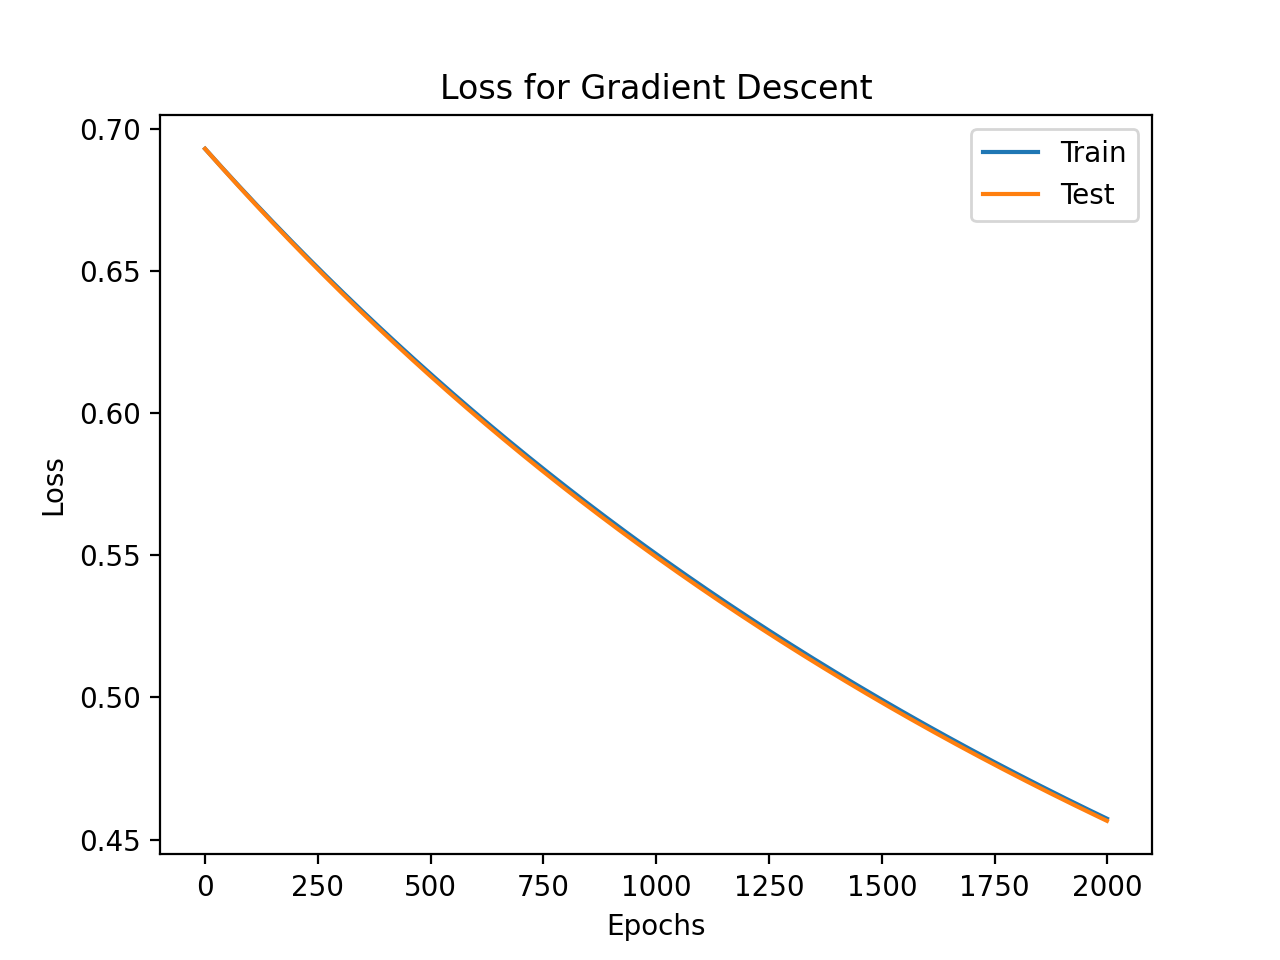
\includegraphics[width=0.5\textwidth]{Figure_1a.png}
            \end{figure}

            \item For both the training set and the test, classify the points according to the rule $\text{sign}(b + x_i^T w)$ and plot the misclassification error as a function of the iteration number (and show both curves on the same plot). 
            
            \begin{figure}[h]
                \centering 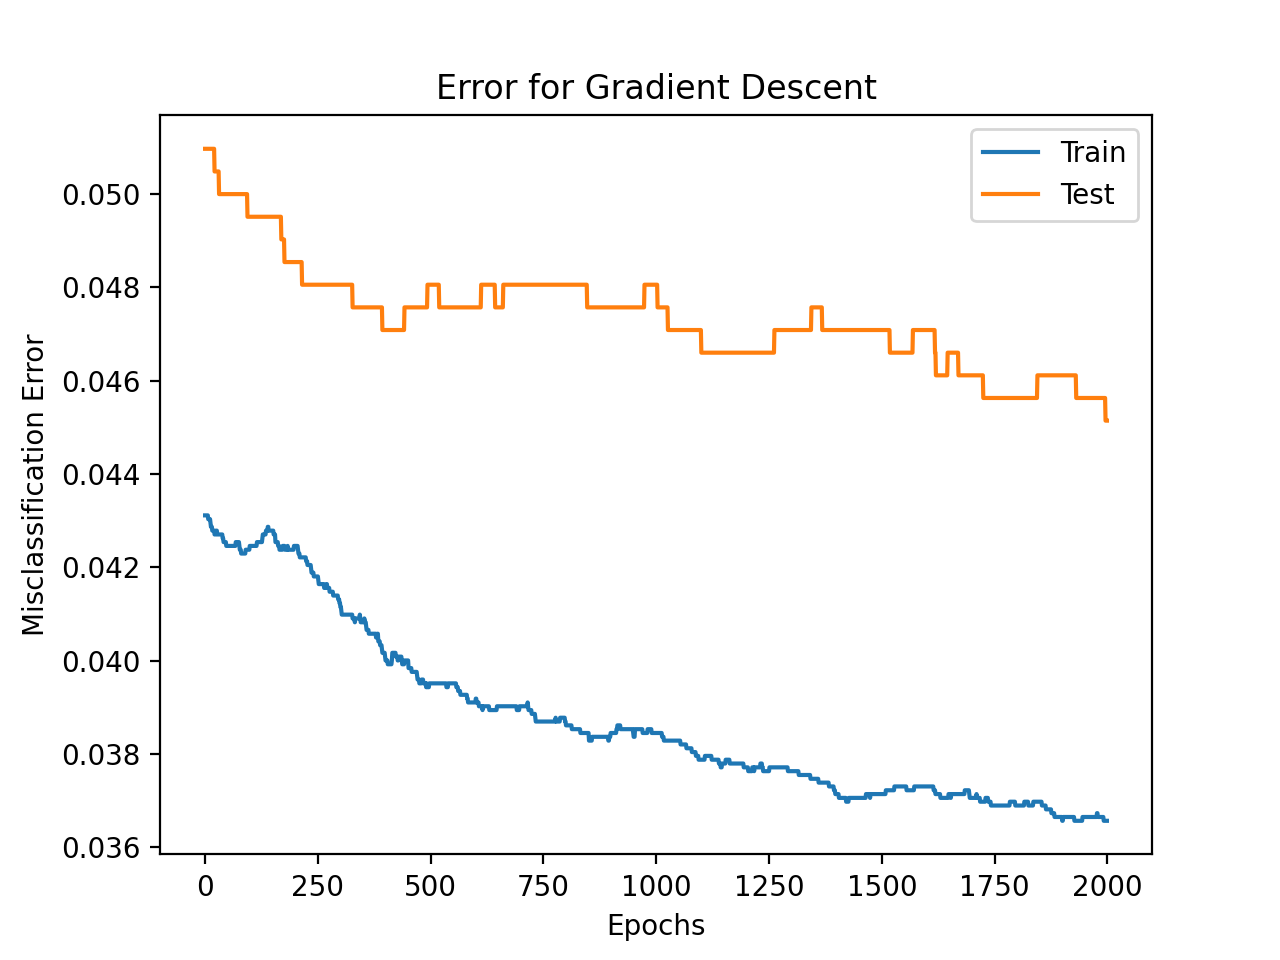
\includegraphics[width=0.5\textwidth]{Figure_1b.png}
            \end{figure}

        \end{enumerate}

        Reminder: Make sure you are only using the test set for evaluation (not for training).
        \newpage

        \item \points{7} Repeat (b) using stochastic gradient descent with a batch size of 1. Note, the expected gradient with respect to the random selection should be equal to the gradient found in part (a). Show both plots described in (b) when using batch size 1. Take careful note of how to scale the regularizer.
        
        \begin{figure}[h]
            \centering 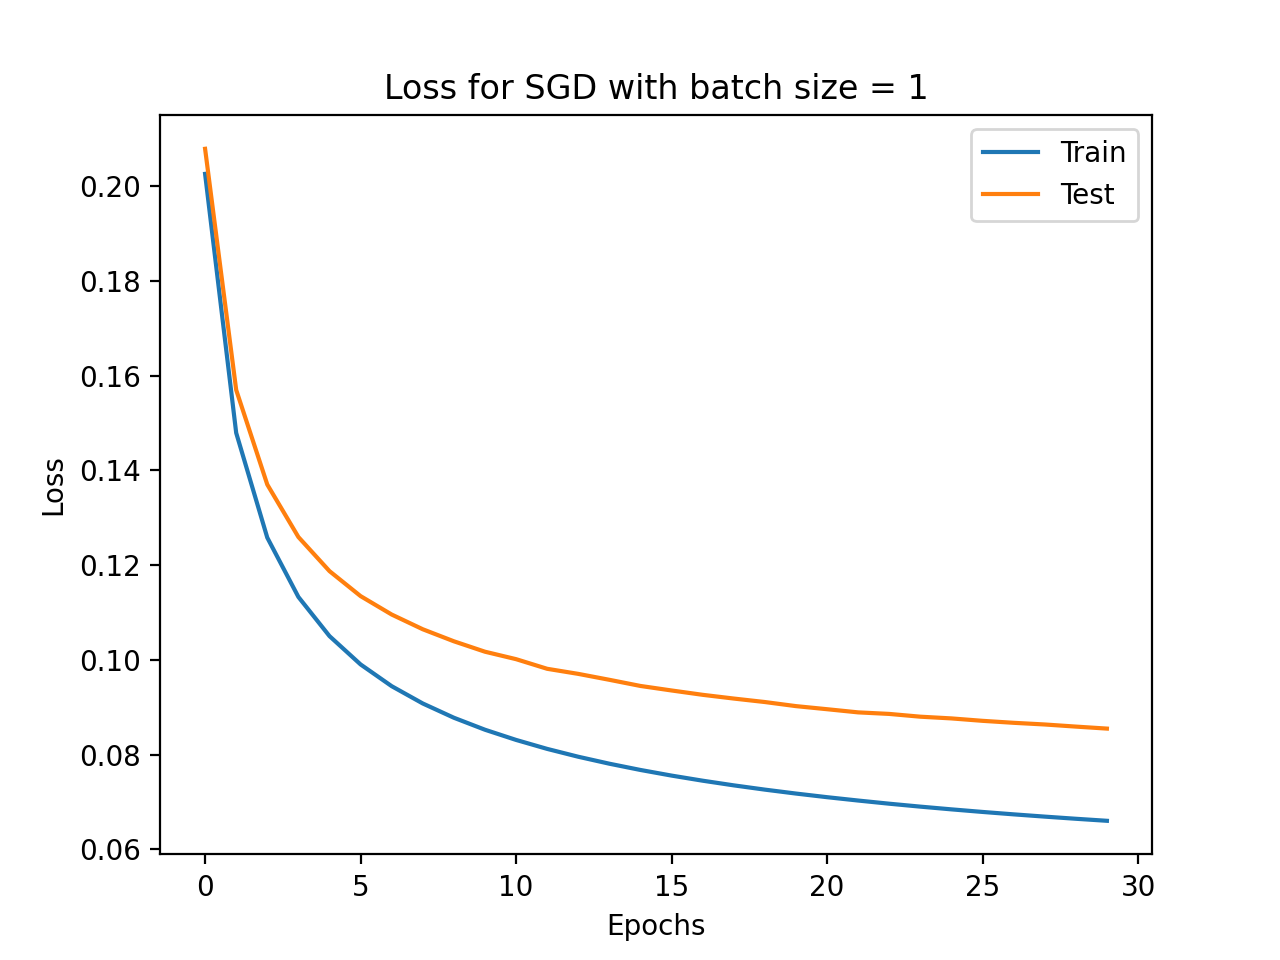
\includegraphics[width=0.5\textwidth]{Figure_1c.png}
        \end{figure}
        \begin{figure}[h]
            \centering 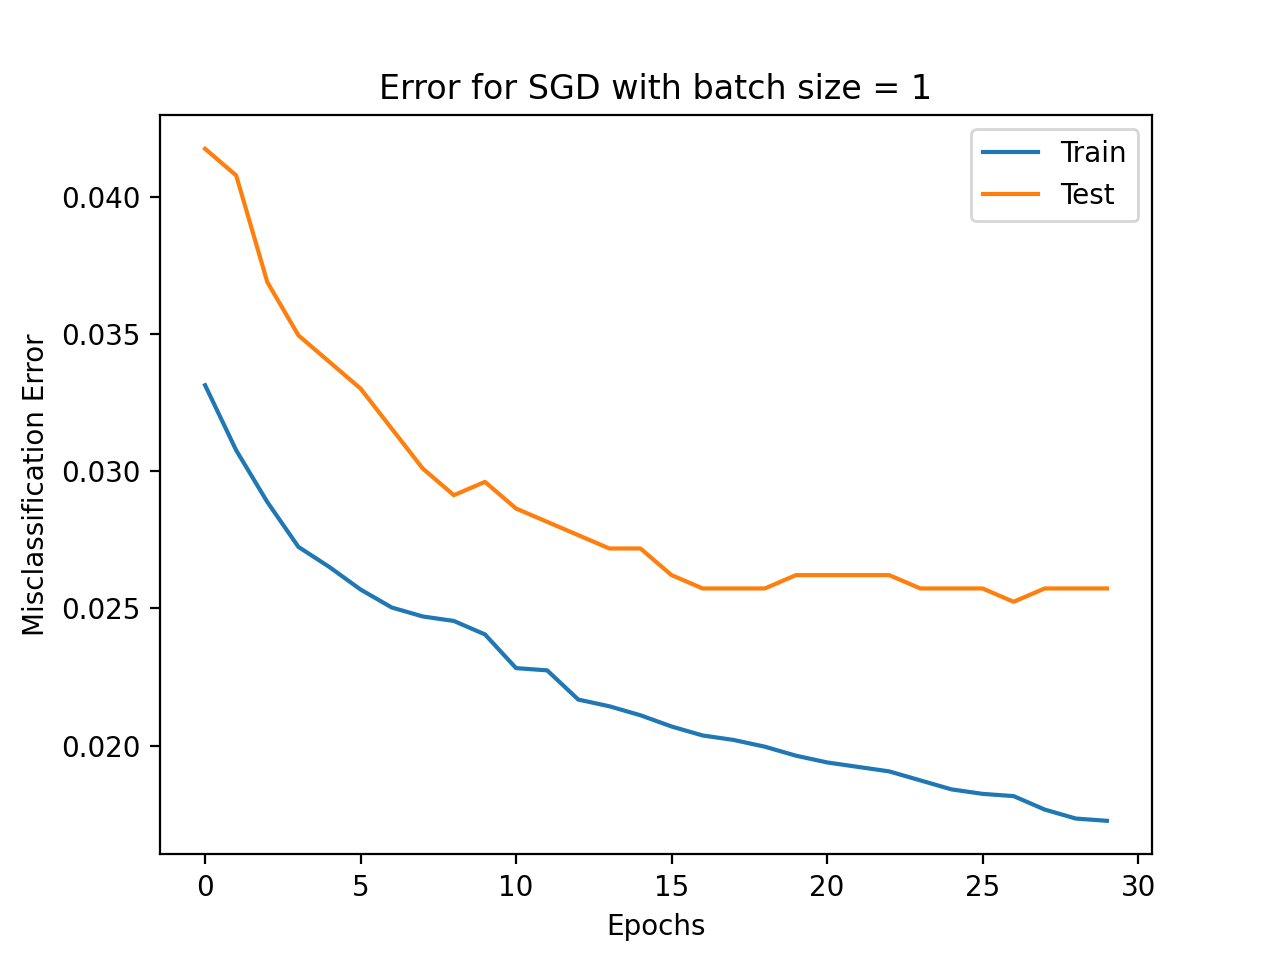
\includegraphics[width=0.5\textwidth]{Figure_1d.png}
        \end{figure}

        \newpage

        \item \points{7} Repeat (b) using stochastic gradient descent with batch size of 100. That is, instead of approximating the gradient with a single example, use 100. Note, the expected gradient with respect to the random selection should be equal to the gradient found in part (a).
        
        \begin{figure}[h]
            \centering 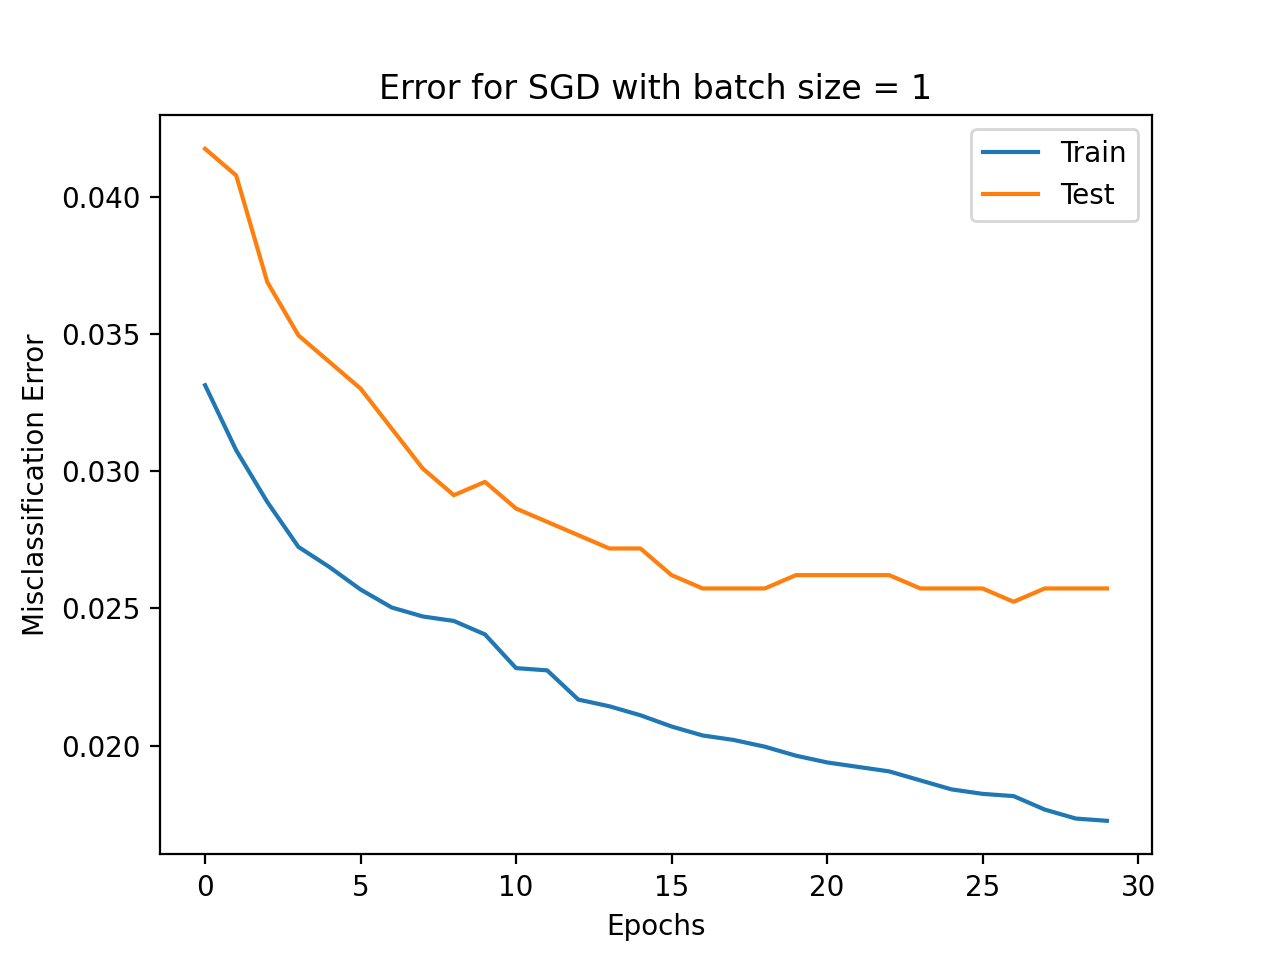
\includegraphics[width=0.5\textwidth]{Figure_1d.png}
        \end{figure}
        \begin{figure}[h]
            \centering 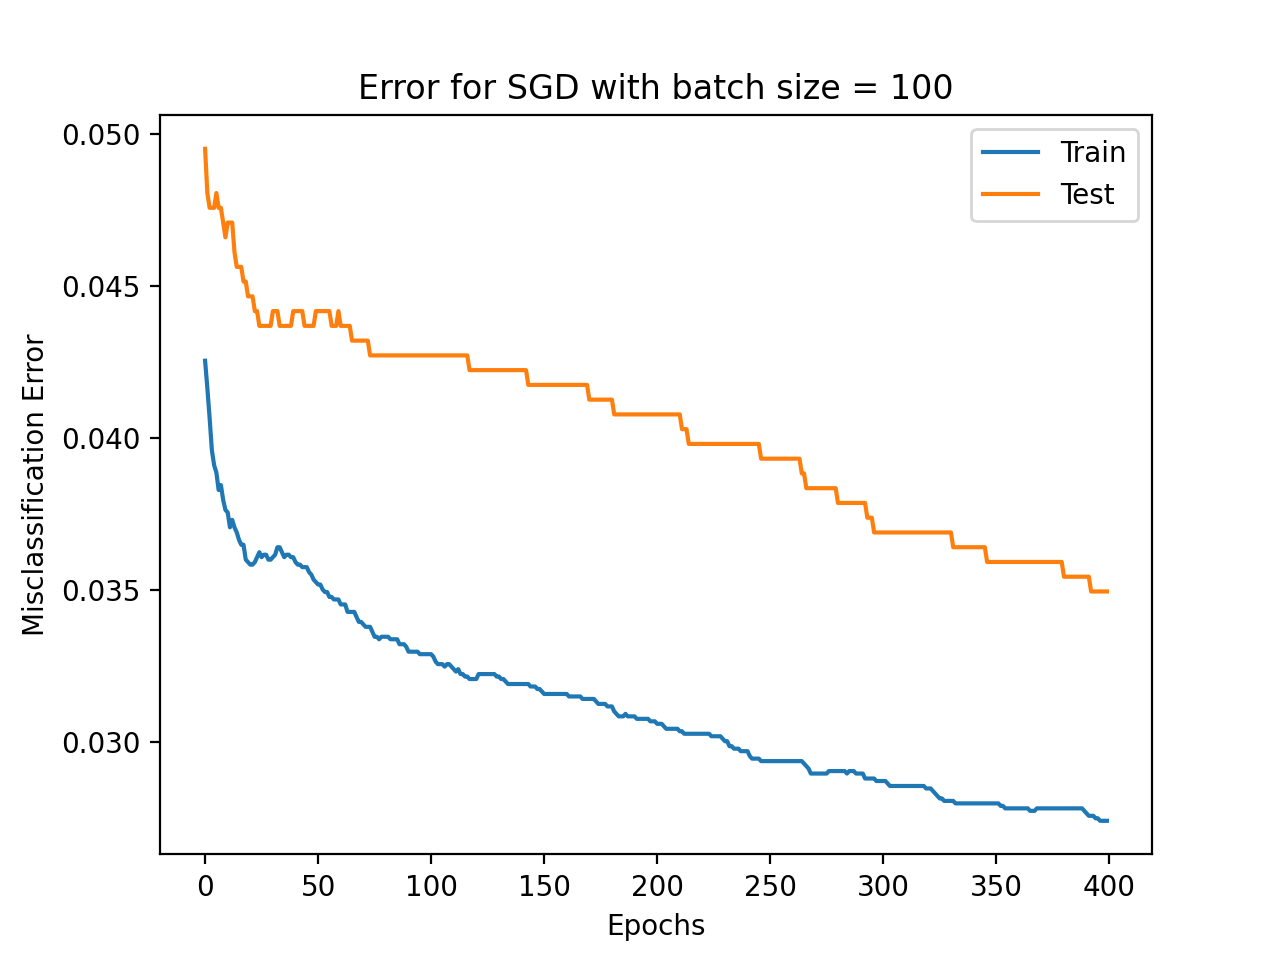
\includegraphics[width=0.5\textwidth]{Figure_1f.png}
        \end{figure}

    \end{enumerate}

\end{aprob}

\newpage
\section*{Ridge Regression on MNIST}

\textbf{These problems were moved from HW1 and are reproduced identically here. If you already started these, you may wish to reuse your work from HW1.}
\begin{aprob}
    In this problem we will implement a regularized least squares classifier for the MNIST data set. The task
    is to classify handwritten images of numbers between $0$ to $9$.\\

    You are \textbf{NOT} allowed to use any of the pre-built  classifiers in \verb|sklearn|.  Feel free to use any method from \verb|numpy| or \verb|scipy|. {\bf Remember:} if you are inverting a matrix in your code, you are probably doing something wrong (Hint: look at \verb|scipy.linalg.solve|).\\

    Each example has features $x_i \in \R^d$ (with $d=28*28=784$) and label $z_j \in \{0,\dots,9\}$. You can visualize a single example $x_i$ with \texttt{imshow} after reshaping it to its original $28 \times 28$ image shape (and noting that the label $z_j$ is accurate). We wish to learn a predictor $\widehat{f}$ that takes as input a vector in $\R^d$ and outputs an index in $\{0,\dots,9\}$. We define our training and testing classification error on a predictor $f$ as
    \begin{align*}
        \widehat{\epsilon}_{\textrm{train}}(f) &=
        \frac{1}{N _{\textrm{train}}} \sum_{(x,z)\in \textrm{Training Set}}     \1\{ f(x) \neq z \}
        \\
          \widehat{\epsilon}_{\textrm{test}}(f) &=
          \frac{1}{N _{\textrm{test}}} \sum_{(x,z)\in \textrm{Test Set}}     \1\{ f(x) \neq z \} 
    \end{align*}

    We will use one-hot encoding of the labels: for each observation $(x,z)$, the original label $z \in \{0, \ldots, 9\}$ is mapped to the standard basis vector $e_{z+1}$ where $e_i$ is a vector of size $k$ containing all zeros except for a $1$ in the $i^{\textrm{th}}$ position (positions in these vectors are indexed starting at one, hence the $z+1$ offset for the digit labels). We adopt the notation where we have $n$ data points in our training objective with features $x_i \in \R^d$ and label one-hot encoded as $y_i \in \{0,1\}^k$. Here, $k=10$ since there are 10 digits.

    \begin{enumerate}
        \item \points{10} In this problem we will choose a linear classifier to minimize the regularized least squares objective:
        \begin{align*}
            \widehat{W} = \text{argmin}_{W \in \R^{d \times k}} \sum_{i=1}^{n} \| W^Tx_{i} - y_{i} \|^{2}_{2} + \lambda \|W\|_{F}^{2}
        \end{align*}
        Note that $\|W\|_{F}$ corresponds to the Frobenius norm of $W$, i.e. $\|W\|_{F}^{2} = \sum_{i=1}^d \sum_{j=1}^k W_{i,j}^2$. To classify a point $x_i$ we will use the rule $\arg\max_{j=0,\dots,9} e_{j+1}^T \widehat{W}^T x_i$. Note that if $W = \begin{bmatrix} w_1 & \dots & w_k \end{bmatrix}$ then
        \begin{align*}
            \sum_{i=1}^{n} \| W^Tx_{i} - y_{i} \|^{2}_{2} + \lambda \|W\|_{F}^{2} &= \sum_{j=1}^k \left[  \sum_{i=1}^n ( e_j^T W^T x_i - e_j^T y_i)^2 + \lambda \| W e_j \|^2 \right] \\
            &= \sum_{j=1}^k \left[  \sum_{i=1}^n ( w_j^T x_i - e_j^T y_i)^2 + \lambda \| w_j \|^2 \right] \\
            &= \sum_{j=1}^k \left[  \| X w_j - Y e_j\|^2 + \lambda \| w_j \|^2 \right]
        \end{align*}
        where $X = \begin{bmatrix} x_1 & \dots & x_n \end{bmatrix}^\top \in \R^{n \times d}$ and $Y = \begin{bmatrix} y_1 & \dots & y_n \end{bmatrix}^\top \in \R^{n \times k}$. Show that
        \begin{align*}
            \widehat{W} = (X^T X + \lambda I)^{-1} X^T Y
        \end{align*}


        \begin{proof}
            We can write the objective as given above: 
            \begin{align*}
                \widehat{W} &= \text{argmin}_{W \in \R^{d \times k}} \sum_{i=1}^{n} \| W^Tx_{i} - y_{i} \|^{2}_{2} + \lambda \|W\|_{F}^{2} \\
                &= \sum_{j=1}^k \left[  \| X w_j - Y e_j\|^2 + \lambda \| w_j \|^2 \right]
            \end{align*}
            if $W = [w_1 \dots w_k]$ and where $X = [x_1 \dots x_n]^\top \in \R^{n \times d}$ and $Y = \begin{bmatrix} y_1 & \dots & y_n \end{bmatrix}^\top \in \R^{n \times k}$. By definition of the norm (dot product),
            \begin{align*}
                \widehat{W} &= \sum_{j=1}^k \left[  \| X w_j - Y e_j\|^2 + \lambda \| w_j \|^2 \right] \\
                &= (X w_j - Y e_j)^\top (X w_j - Y e_j) + \lambda w_j^\top w_j \\
            \end{align*}
            To get the arg min, we can take the derivative and set it to zero.
            \begin{align*}
                0 =& \frac{\diff}{\diff w_j} \left[ (X w_j - Y e_j)^\top (X w_j - Y e_j) + \lambda w_j^\top w_j \right] \\
                0 &= 2X^\top (X w_j - Y e_j) + 2 \lambda w_j \\
                0 &= X^\top X w_j - X^\top Y e_j + \lambda w_j \\
                X^\top Y e_j &= X^\top X w_j + \lambda I_d w_j \\
                X^\top Y e_j &= (X^\top X + \lambda I_d) w_j \\
                w_j &= (X^\top Y e_j)(X^\top X + \lambda I_d)^{-1}\\
            \end{align*}
            Because $e_j$ is the basis vector then $Y e_j$ is the $j$th column of $Y$, then 

            \begin{align*}
                \widehat{W} &= [ w_1 \dots w_k ] \\
                &=  [(X^\top Y e_1)(X^\top X + \lambda I_d)^{-1} \dots (X^\top Y e_k)(X^\top X + \lambda I_d)^{-1}] \\
                &=  (X^\top X + \lambda I_d)^{-1}) X^\top [Y e_1  \dots Y e_k] \\
                &=  (X^\top X + \lambda I_d)^{-1}) X^\top Y \\
            \end{align*}
        \end{proof}

        \newpage
        \item \points{10}
        \begin{itemize}
            \item Implement a function \verb|train| that takes as input $X \in\R^{n \times d}$, $Y \in \{0,1\}^{n \times k}$, $\lambda > 0$ and returns $\widehat{W} \in \R^{d \times k}$.
            \item Implement a function \verb|one_hot| that takes as input $Y \in \{0, ..., k-1\}^{n}$, and returns $Y \in \{0,1\}^{n \times k}$.
            \item Implement a function  \verb|predict| that takes as input $W \in \R^{d \times k}$, $X' \in\R^{m \times d}$ and returns an $m$-length vector with the $i$th entry equal to $\arg\max_{j=0,\dots,9} e_j^T W^T x_i'$ where $x_i' \in \R^d$ is a column vector representing the $i$th example from $X'$.
            \item Using the functions you coded above, train a model to estimate $\widehat{W}$ on the MNIST training data with $\lambda = 10^{-4}$, and make label predictions on the test data. This behavior is implemented in \verb|main| function provided in zip file. {\bf What is the training and testing error?} Note that they should both be about $15\%$. 
        \end{itemize}
    \end{enumerate}

    \subsubsection*{Solution:}
    \begin{itemize}
        \item The error output from my implementation is 15 \% for both training and test error. More specifically, train error is 14.805 \% and the test error is 14.66 \%. 
    \end{itemize}
\end{aprob}

\newpage
\begin{bprob}
    \begin{enumerate}

        \item \points{5} Instead of reporting just the test error, which is an unbiased estimate of the \emph{true} error, we would like to report a \emph{confidence interval} around the test error that contains the true error.
        \begin{lemma}(Hoeffding's inequality)
            Fix $\delta \in (0,1)$. If for all $i=1,\dots,m$ we have that $X_i$ are i.i.d. random variables with $X_i \in [a,b]$ and $\mathbb{E}[X_i] = \mu$ then
            \begin{align*}
                \P\left( \left| \left(\frac{1}{m} \sum_{i=1}^m X_i\right) - \mu \right| \geq \sqrt{\frac{(b-a)^2\log(2/\delta)}{2m}} \right) \leq \delta
            \end{align*}
        \end{lemma}
        We will use the above equation to construct a confidence interval around the true classification error $\epsilon(\widehat{f})=\mathbb{E}_{\text{test}}[\widehat{\epsilon}_{\textrm{test}}(\widehat{f})]$ since the test error $\widehat{\epsilon}_{\textrm{test}}(\widehat{f})$ is just the average of indicator variables taking values in $\{0,1\}$ corresponding to the $i$th test example being classified correctly or not, respectively, where an error happens with probability $\mu=\epsilon(\widehat{f})=\mathbb{E}_{\text{test}}[\widehat{\epsilon}_{\textrm{test}}(\widehat{f})]$, the \emph{true} classification error. 
        
        Let $\widehat{p}$ be the value of $p$ that approximately minimizes the validation error on the plot you just made and use $\widehat{f}(x) = \arg\max_j x^T \widehat{W}^{\widehat{p}} e_j$ to compute the classification test error $\widehat{\epsilon}_{\textrm{test}}(\widehat{f})$. Use Hoeffding's inequality, of above, to compute a confidence interval that contains $\mathbb{E}_{\text{test}}[\widehat{\epsilon}_{\textrm{test}}(\widehat{f})]$ (i.e., the \emph{true} error) with probability at least $0.95$ (i.e., $\delta=0.05$). Report $\widehat{\epsilon}_{\textrm{test}}(\widehat{f})$ and the confidence interval. 
    \end{enumerate}
    
    \subsubsection*{Solution:}
    \begin{itemize}
        \item \textbf{Part a:} The testing error is the same as from A5 (b), that is 14.66 \%. We find the confidence interval is  0.00554442622077. 
        
        Since the data is from 0 to 1, $a=0$ and $b=1$. Let's also find 
        $$ \widehat{\epsilon}_{\textrm{test}}(\widehat{f}) = \frac{1}{m} \sum_{i=1}^m X_i $$
        So, the test error $\widehat{\epsilon}_{\textrm{test}}(\widehat{f}) $ is just the mean of the $i$th column of $X$. In other words, 
        \begin{equation*}
            \widehat{\epsilon}_{\textrm{test}}(\widehat{f}) = \frac{1}{m} \sum_{i=1}^m (\widehat{f}(x_i) = y_i)
        \end{equation*}
        This works in general since $X$ is i.i.d. Then Hoeffding's inequality is 
        \begin{equation*}
            \P\left( \left| \left( \widehat{\epsilon}_{\textrm{test}}(\widehat{f}) \right)- \mu \right| \geq \sqrt{\frac{(b-a)^2\log(2/\delta)}{2m}} \right) \leq \delta
        \end{equation*}
        \begin{equation*}
            \implies \P\left( \left| \left( \widehat{\epsilon}_{\textrm{test}}(\widehat{f}) \right)- \mu \right| \geq \sqrt{\frac{(\log(2/0.05)}{2m}} \right) \leq 0.05
        \end{equation*}
        Thus, the confidence interval to 95 \% is given by 
        $$ \epsilon(\widehat{f}) \in (\widehat{\epsilon}(\widehat{f})\pm |v|) $$ 
        where $ v = \sqrt{\frac{(\log(2/0.05)}{2m}} $. In this case, $m = 60,000$, so 
        the confidence interval, $v$ is 
        $$ v = \sqrt{\frac{(\log(2/0.05)}{2\cdot 60000}} =  0.00554442622077 $$
    \end{itemize}
\end{bprob}

\newpage
\section*{Confidence Interval of Least Squares Estimation}
\subsection*{Bounding the Estimate} 
\begin{bprob}
    Let us consider the setting, where we have $n$ inputs, $X_1, ..., X_n \in \R^d$, and $n$ observations $Y_i = \langle X_i, \beta^* \rangle + \epsilon_i$, for $i = 1, ..., n$. Here, $\beta^*$ is a ground truth vector in $\R^d$ that we are trying to estimate, the noise $\epsilon_i \sim \mathcal{N}(0, 1)$, and the $n$ examples piled up --- $X \in R^{n\times d}$. To estimate, we use the least squares estimator $\widehat{\beta} = \min_\beta \lVert X\beta - Y\rVert_2^2$. Moreover, we will use $n=20000$ and $d=10000$ in this problem.

    \begin{enumerate}
        \item \points{3} Show that $\widehat{\beta}_j \sim \mathcal{N}(\beta_j^*, (X^T X)^{-1}_{j, j})$ for each $j = 1, ..., d$. \emph{(Hint: see notes on confidence intervals from lecture.)}
        \begin{proof}
            From lecture, we have
            \begin{align*}
                \widehat{\beta} &= (X^\top X)^{-1} X^\top Y \\
                &= (X^\top X)^{-1} X^\top (X \beta^* + \epsilon ) \\
                &= \beta^*  + (X^\top X)^{-1} X^\top \epsilon \\
                \widehat{\beta} - \beta^* &= (X^\top X)^{-1} X^\top \epsilon
            \end{align*}
            From class notes, we can use Proposition 1 to write the Gaussian in $p$ dimensions with $ \epsilon = \mathcal{N}(0,I_d)$.
            \begin{align*}
                \widehat{\beta} &\sim \mathcal{N}(0 \cdot \beta^*  + (X^\top X)^{-1} X^\top \epsilon,  (X^\top X)^{-1} X^\top I_d ((X^\top X)^{-1} X^\top)^\top ) \\
                &= \mathcal{N}( \beta^*, (X^\top X)^{-1} X^\top X (X^{-1} X^{-\top} )^\top )\\
                & = \mathcal{N}( \beta^*, (X^\top X)^{-1} (X^{-1} X^{-\top} )^\top )\\
                & = \mathcal{N}( \beta^*, (X^{\top} X)^{-1} ) \\
            \end{align*}
            This is the full matrix of $\widehat{\beta}$, so if we want the $j$th element then we take the $j$th diagonal from the matrix $(X^\top X)^{-1}$ sicne this is a square symmetric matrix. Hence,
            $$ \widehat{\beta}_j \sim \mathcal{N} (\beta^*_j, (X^\top X)^{-1}_{j,j}) $$

        \end{proof}
        \newpage
        \item \points{4} Fix $\delta \in (0,1)$ suppose $\beta^* = 0$. Applying the proposition from the notes, conclude that for each $j \in [d]$, with probability at least $1-\delta$, $|\widehat{\beta}_j| \leq \sqrt{2(X^TX)^{-1}_{j, j} \log(2 / \delta)}$.
        Can we conclude that with probability at least $1-\delta$,  $|\widehat{\beta}_j| \leq \sqrt{2(X^TX)^{-1}_{j, j} \log(2 / \delta)}$ for all $j \in [d]$ simultaneously? Why or why not?
        
        N/A
        
        \item \points{5} Let's explore this question empirically. Assume data is generated as $x_i = \sqrt{(i \mod d) + 1} \cdot e_{(i \mod d) + 1}$ where $e_i$ is the $i$th canonical vector and $i \mod d$ is the remainder of $i$ when divided by $d$. Generate each $y_i$ according to the model above. 
        Compute $\widehat{\beta}$ and plot each $\widehat{\beta}_j$ as a scatter plot with the $x$-axis as $j \in \{1,\dots,d\}$. Plot $\pm \sqrt{2(X^TX)^{-1}_{j, j} \log(2 / \delta)}$ as the upper and lower confidence intervals with $1 - \delta = 0.95$. How many $\widehat{\beta}_j$'s are outside the confidence interval?  \emph{Hint: Due to the special structure of how we generated $x_i$, we can compute $(X^TX)^{-1}$ analytically without computing an inverse explicitly.}

        N/A
        
    \end{enumerate}

\end{bprob}

\newpage
\section*{Administrative}
\begin{aprob}
\begin{enumerate}
    \item \points{2} About how many hours did you spend on this homework? There is no right or wrong answer :)
\end{enumerate}

\subsection*{Answer:}
About 12-16 hours

\end{aprob}

\end{document}
